\paragraph{Алгоритм обнаружения и оценки параметров ШПС в условиях интерференции (DMA + уточненный АР)}

В данной работе предлагается объединить результаты работы алгоритма DMA, рассмотренного в
\cite{tsui, lin_dma} и, предложенных в данной работе, усовершенствованного итеративного 
алгоритма уточнения АКФ гармонического сигнала и подхода для оценки частоты ПСП-модулированного
сигнала при помощи АР-модели.

Схематично приемник изображен на рисунке \ref{pic:ar_dma_scheme}

\begin{figure}[H]
\center\scalebox{1}{\includegraphics[width=1\linewidth]{dma_quadruple_lpc.eps}}
	\caption{Алгоритм обнаружения и оценки параметров ШПС в условиях интерференции (DMA + уточненный АР)}
	\label{pic:ar_dma_scheme}
\end{figure}

Выходом алгоритма DMA является оценка фазы ПСП. Повторно модулируя входящий сигнал ПСП с полученной
фазой, можно восстановить гармонический сигнал. Для оценки частоты данного сигнала применяется
АР-метод. Но для оценки АР-методом, требуется точная оценка АКФ, которую можно получить
с помощью усовершенствованного итеративного алгоритма вычисления АКФ.

%Рекомендации по выбору задержки ${\tau}$ и детали алгоритма DMA рассмотрены в разделе
%\ref{sec1:dma_real}.

Предложенный алгоритм можно описать следующим набором шагов:
\begin{itemize}
\item[Шаг 1.] Входной сигнал ${x(k)}$ умножается на задержанную копию ${x(t-\tau)}$. Так же
	на данном шаге можно производить когерентное накопление результата, для
	увеличения ОСШ.

	\begin{center}
	\begin{equation}
		%\label{}
		x_{new}(k) = \frac{C_{new}(k)}{2} \left(\cos (2\pi f \tau) - \cos \left[2 \pi f (2t - \tau)\right]\right)
	\end{equation}
	\end{center}

\item[Шаг 2.] Полученный сигнал ${x_{new}(k)}$ фильтруется ФВЧ для отсечения высокочастотной компоненты.
\item[Шаг 3.] Генерируется локальная ПСП ${C(k)}$ и умножается на задержанную копию ${C(k-\tau)}$.

	\begin{center}
	\begin{equation}
		%\label{}
		C_{new}(k) = C(k)C(k-\tau)
	\end{equation}
	\end{center}

\item[Шаг 4.] Отфильтрованный сигнал ${x_{filt}(k)}$ коррелируется с новой ПСП ${C_{new}(k)}$
	с использованием БПФ. Выход коррелятора сравнивается с заранее определенным порогом.

	\begin{center}
	\begin{equation}
		%\label{}
		x_{filt}(k) = \frac{C_{new}(k)}{2} \cos (2\pi f \tau)
	\end{equation}
	\end{center}

	\subitem{\bf{Если}}  значение оказалось больше порогового {\bf{то}},
		принимается решение о наличии сигнала. Полученное значение фазы ПСП  - ${m}$ запоминается.
		Перейти на шаг 5.
	\subitem{\bf{Иначе}} 
		Принимается решение об отсутствии сигнала.
\item[Шаг 5.] Входной сигнал ${x(k)}$ модулируется ПСП ${C(k-m)}$. В результате получаем гармонический
	сигнал ${x_{cos}(k)}$ с неизвестной частотой.
\item[Шаг 6.] Для увеличения ОСШ сигнала ${x_{cos}(k)}$ вычисляется значение уточненное значение АКФ
	по усовершенствованному итеративному алгоритму получения АКФ.
\item[Шаг 7.] Определяются коэффициенты АР-модели ${\hat{a_1}, \hat{a_2}}$, по формуле \ref{eq:ar_coef_matrix}.
	Вычисляется резонансная частота ${\omega_0 = 2 \pi f}$ и определяется квадрат модуля частотного отклика АР-модели для этой частоты. 
\end{itemize}

Количество итераций требуемых для оценки частоты одного источника:
\begin{enumerate}
\item Алгоритм DMA:
	\begin{center}
	\begin{equation}
		%\label{}
		OP_{DMA} = 8NlogN + 6N
	\end{equation}
	\end{center}

\item Усовершенствованный итеративный алгоритм получения АКФ:
	\begin{center}
	\begin{equation}
		%\label{}
		OP_{ACF} = 8NlogN + (k+2)N
	\end{equation}
	\end{center}
	
\item Вычисление полюсов передаточной функции АР-модели:
	\begin{center}
	\begin{equation}
		%\label{}
		OP_{AR} = 51
	\end{equation}
	\end{center}

\end{enumerate}

Следует отметить, что в пункте 3 произведены допущения: стоимость 1 операции деления равна 10 операциям умножения,
стоимость операции извлечения корня составляет 20 операций умножения, стоимость сложения не учитывается.

%Количество итераций требуемых для оценки частоты одного источника параллельным корррелятором:
